\subsection{Letter Recognition}

\subsubsection{Backpropagation padrão}

O backpropagation padrão foi executado para a base de dados Letter Recognition com os seguintes parâmetros:

\begin{itemize}
	\item \texttt{size}: 10
	\item \texttt{learnFuncParams}: 0.1
	\item \texttt{maxit}: 100
\end{itemize}

A confusion matrix de uma execução é apresentada na Figura \ref{figura-confusion-matrix-letter-recognition-backpropagation-padrao}.

\begin{figure}[h!]
  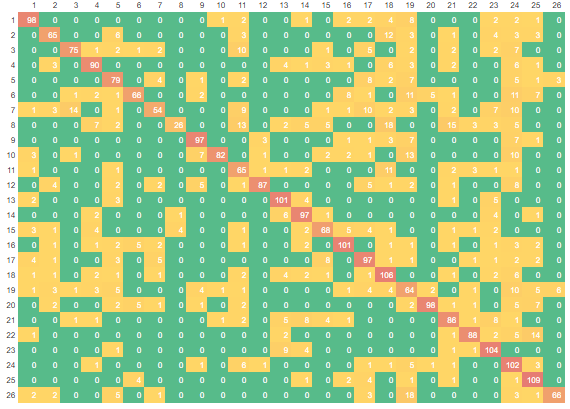
\includegraphics[width=\linewidth]{figs/confusion-matrix-letter-recognition-backpropagation-padrao.png}
  \caption{Confusion Matrix - Letter Recognition - Backpropagation padrão}
  \label{figura-confusion-matrix-letter-recognition-backpropagation-padrao}
\end{figure}

Os resultados para as 10 execuções do backpropagation padrão com as taxas de acertividade são apresentados na Tabela \ref{tabela-resultado-letter-recognition-backpropagation-padrao}. A média de acertividade foi de $0.7391$, com desvio padrão de $0.0062$.

\begin{table}[h!]
\centering
\caption{Resultados - Letter Recognition - Backpropagation padrão}
\label{tabela-resultado-letter-recognition-backpropagation-padrao}
\begin{tabular}{ll}
\toprule
                       & \textbf{Acertividade}       \\ \midrule
Execução 1             & 0.7363          \\
Execução 2             & 0.7370          \\
Execução 3             & 0.7380          \\
Execução 4             & 0.7527           \\
Execução 5             & 0.7360          \\
Execução 6             & 0.7353           \\
Execução 7             & 0.7367           \\
Execução 8             & 0.7477          \\
Execução 9             & 0.7380           \\
Execução 10            & 0.7330           \\ \bottomrule
\textbf{Média}         & \textbf{0.7391} \\
\textbf{Desvio Padrão} & \textbf{0.0062}
\end{tabular}
\end{table}

%O erro iterativo é apresentado na Figura \ref{figura-erro-iterativo-letter-recognition-backpropagation-padrao}.
%
%\begin{figure}
%  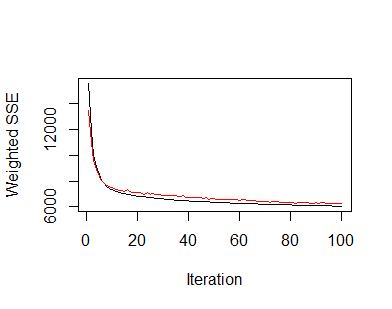
\includegraphics[width=\linewidth]{figs/erro-iterativo-letter-recognition-backpropagation-padrao.png}
%  \caption{Erro iterativo - Letter Recognition - Backpropagation padrão}
%  \label{figura-erro-iterativo-letter-recognition-backpropagation-padrao}
%\end{figure}

\subsubsection{SCG}

O backpropagation com função de aprendizado SCG foi executado para a base de dados Letter Recognition com os seguintes parâmetros:

\begin{itemize}
	\item \texttt{size}: 10
	\item \texttt{learnFuncParams}: (0, 0, 0, 0)
	\item \texttt{maxit}: 100
\end{itemize}

A confusion matrix de uma execução é apresentada na Figura \ref{figura-confusion-matrix-letter-recognition-backpropagation-scg}.

\begin{figure}[h!]
  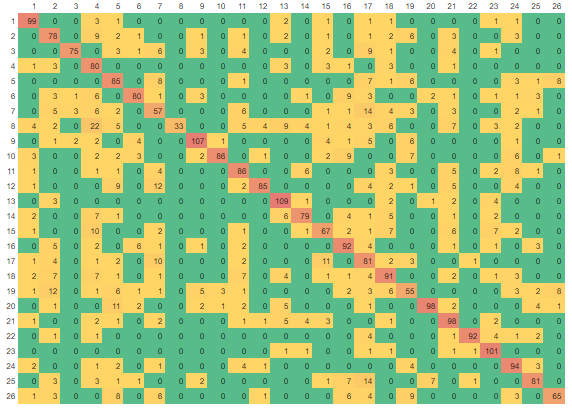
\includegraphics[width=\linewidth]{figs/confusion-matrix-letter-recognition-backpropagation-scg.png}
  \caption{Confusion Matrix - Letter Recognition - Backpropagation SCG}
  \label{figura-confusion-matrix-letter-recognition-backpropagation-scg}
\end{figure}

Os resultados para as 10 execuções do backpropagation SCG com as taxas de acertividade são apresentados na Tabela \ref{tabela-resultado-letter-recognition-scg}. A média de acertividade foi de $0.7262$, com desvio padrão de $0.0112$.

\begin{table}[h!]
\centering
\caption{Resultados - Letter Recognition - Backpropagation SCG}
\label{tabela-resultado-letter-recognition-scg}
\begin{tabular}{ll}
\toprule
                       & \textbf{Acertividade}       \\ \midrule
Execução 1             & 0.7430          \\
Execução 2             & 0.7280          \\
Execução 3             & 0.7187           \\
Execução 4             & 0.7117          \\
Execução 5             & 0.7203           \\
Execução 6             & 0.7327          \\
Execução 7             & 0.7163           \\
Execução 8             & 0.7257           \\
Execução 9             & 0.7207          \\
Execução 10            & 0.7453          \\ \bottomrule
\textbf{Média}         & \textbf{0.7262} \\
\textbf{Desvio Padrão} & \textbf{0.0112}
\end{tabular}
\end{table}

%O erro iterativo é apresentado na Figura \ref{figura-erro-iterativo-letter-recognition-backpropagation-scg}.
%
%\begin{figure}
%  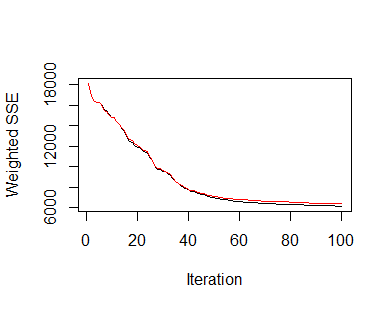
\includegraphics[width=\linewidth]{figs/erro-iterativo-letter-recognition-backpropagation-scg.png}
%  \caption{Erro iterativo - Letter Recognition - Backpropagation SCG}
%  \label{figura-erro-iterativo-letter-recognition-backpropagation-scg}
%\end{figure}